\documentclass{article} % For LaTeX2e
\usepackage{iclr2016_conference,times}
\usepackage{hyperref}
\usepackage{url}
\usepackage{graphicx}
\usepackage{tabularx,ragged2e,booktabs,caption}
\usepackage[utf8]{inputenc}

\title{8-Bit Approximations for Parallelism in Deep Learning}


\author{Tim Dettmers \\
The Faculty of Informatics\\
Universià della Svizzera italiana\\
Via Giuseppe Buffi 13, CH-6904 Lugano, Switzerland \\
\texttt{tim.dettmers@gmail.com} 
}

% The \author macro works with any number of authors. There are two commands
% used to separate the names and addresses of multiple authors: \And and \AND.
%
% Using \And between authors leaves it to \LaTeX{} to determine where to break
% the lines. Using \AND forces a linebreak at that point. So, if \LaTeX{}
% puts 3 of 4 authors names on the first line, and the last on the second
% line, try using \AND instead of \And before the third author name.

\newcommand{\fix}{\marginpar{FIX}}
\newcommand{\new}{\marginpar{NEW}}

%\iclrfinalcopy % Uncomment for camera-ready version

\begin{document}


\maketitle

\begin{abstract}
The creation of practical deep learning data-products often requires the parallelization across processors and computers to make deep learning feasible on large data sets, but bottlenecks in communication bandwidth make it difficult to attain good speedups through parallelism. Here we develop and test 8-bit approximation algorithms, which provide improved utilization of the available bandwidth by compressing 32-bit gradients and nonlinear activations to 8-bit approximations. We show that these approximations do not decrease predictive performance on MNIST, CIFAR10, and ImageNet for both model and data parallelism and provide a data transfer speedup of 2x relative to 32-bit parallelism. We also show that 8-bit approximations can increase training speed and performance in very deep networks which use rectified linear units. We compare our data types with other methods and show that 8-bit approximations achieve state-of-the-art speedups for model parallelism in general and data parallelism with up to 200k parameters per layer. Thus 8-bit approximation is the single best method for parameter compression in the parallelization of convolutional networks.
\end{abstract}

\section{Introduction}
Deep learning is a field inherently driven by advances in computational processing \citep{schmidhuber2015deep}. Graphics processing units (GPUs) can accelerate deep learning by a factor of up to 50 compared to a normal processor (CPU), and these speedups were integral in achieving breakthroughs in speech recognition and computer vision \citep{ciresan2012multi, dahl2012context,krizhevsky2012imagenet}. After these breakthroughs, GPUs found widespread use and many teams sought to accelerate the training of deep learning algorithms further by parallelizing the training procedure across multiple GPUs or computers \citep{chilimbi2014project,coates2013deep,dean2012large,wu2015deep}. To make deep learning applicable and scalable for large data sets, it is important to develop successful parallel deep learning algorithms.

The main difficulty in the parallelization of deep learning is the sequential nature of backpropagation where the parameter updates must be fully completed before the next iteration of stochastic gradient descent can ensue \citep{rumelhart1988learning}. This creates an environment where transfer of parameters between GPUs and computers require high bandwidth and low latency for network communication. Network communication generally constitutes the major bottleneck in deep learning parallelism.

There are two major ways to increase the performance of a parallel deep learning algorithm: (1) Overlap communication and computation in such a way that most of the communication is done while we wait for a computation to finish; (2) Decrease the number or size of parameters needed to transfer;

In this paper we work on (2) and make the following contributions: 
\begin{itemize}
	\item We discuss all important hardware and software bottlenecks in model and data parallel deep learning algorithms on GPUs
	\item We develop 8-bit gradient approximation data types and by applying them to MNIST, CIFAR10 and ImageNet show that the error rates remain unchanged despite this approximation
	\item We show that speedup gains of 8-bit approximation compared to 32-bit transfers lie between 1.5-2.1 for common gradient dimensions in deep learning architectures
	\item We compare our algorithm with similar work and show that 8-bit approximation sets the state-of-the-art for model parallelism in general and for data parallelism with less than 200000 parameters per layer
	\item We show and investigate an effect where 8-bit approximation for model parallelism in conjunction with RMSProp yields superior performance in deep networks compared to 32-bit training
\end{itemize}
\section{Background}

 To understand the properties of a successful parallel deep learning algorithm, it is necessary to understand how the communication between GPUs works and what the bottlenecks for both model and data parallelized deep learning architectures are. First we look at the specific properties of data and model parallelism, and then we look at general bottlenecks in GPU-to-GPU communication.

\subsection{Data parallelism}

In data parallelism, the model is kept constant for all GPUs while each GPU is fed with a different mini-batch. After each pass the gradients are exchanged, i.e. synchronized with each GPU:
\begin{itemize} 	
	\item How it is done: For densely connected layers, data is split by the sample dimension, e.g. for 4 GPUs, a 1024x784 mini-batch is split into four 256x784 batches; for convolutional layers the data is split by the sample dimension (better cross-validation error), or by the feature map dimension (decreases memory usage dramatically; slightly worse cross-validation error; makes architecture complicated)
	\item Infrequent synchronization: Parameters are synchronized (averaged) once after each full forward+backward pass
	\item Efficiency: Data parallelism is efficient when the model has few parameters, e.g. long short-term memory recurrent neural networks \citep{hochreiter1997long}; or the computational costs per parameter are high, e.g. convolutional layers in convolutional nets
	\item Scaling limitations: Current GPU implementations are optimized for larger matrices so data parallelism does not scale indefinitely due to slow matrix operations (especially matrix multiplication) for small mini-batch sizes ($< 128$ per GPU); convolution implementations that rely on matrix multiplication may suffer from this too
	\item Requires asymptotic accuracy: Good solutions can be found as long as the sequence of updates converges to the minimum asymptotically \citep{seide20141}
\end{itemize}

\subsection{Model parallelism}
In model parallelism the data is kept constant for all GPUs while each GPU holds only a part of the full model:
\begin{itemize}
	\item How it is done: Distribute the parameters of a layer on multiple GPUs (split by input or output dimension); pass the same mini-batch through the distributed layer
	\item Frequent synchronization: Parameters are synchronized once every layer; the outputs of the layer are either stacked or added together depending on the matrix operation
	\item Efficiency: Model parallelism is efficient when the layer has many parameters, e.g. in densely connected layers (because the parameter matrix is reduced by a factor equal to the number of GPUs)
	\item Scaling limitations: Poor performance for larger mini-batch sizes; the larger the mini-batch size, the larger the matrix that needs to be synchronized across GPUs
	\item Requires numerical accuracy: Outputs must be precise as small deviation may lead to large errors in later layers; this is similar to the exploding gradient problem \citep{hochreiter2001gradient}
\end{itemize}

\subsection{General bottlenecks}

\subsubsection{PCIe switches}

PCI Express (PCIe) is built like an ordinary network where pairs of two PCIe slots share a common switch which can serve one outgoing and incoming connection simultaneously. Thus only a single device in a device-pair can communicate with another another device-pair at any one time. This holds for both GPUs and InfiniBand cards. Thus PCIe switches need to be taken into account to obtain optimal performance in a multi-GPU system.

\subsubsection{Bandwidth and latency}
GPUs within a computer communicate by using the PCIe interface which offers about 7 GB/s practical performance when a computer contains more than 2 GPUs and about 14 GB/s when it contains 2 GPUs. 

GPUs between computers usually communicate by using InfiniBand network cards which have a practical bandwidth of 3-7GB/s (quad-data-rate (QDR) and fourteen-data-rate cards (FDR), respectively).

Both PCIe and InfiniBand communication usually have about 1-2ms latency per layer for deep learning sized data transfers (as a comparison: adding two matrices for a layer of this size takes about 0.05-0.1ms on a GPU). Note that both bandwidth and latency are smaller for small messages. 

Communication is the main bottleneck in deep learning which can be illustrated with a simple example: AlexNet is a convolutional network with about 60 million parameters \citep{krizhevsky2012imagenet}; a full forward-backward pass is completed in under 100ms for current generation GPUs\footnote{https://github.com/soumith/convnet-benchmarks}. With 4 GPUs in naive data parallelism we need to synchronize 60 million parameters with the 3 other GPUs. Due to PCIe switches over which GPU pairs have to send their messages, this takes as long as sending 4 messages between 2 unpaired GPUs. Now 60 million 32-bit parameters take up 0.223GB of memory which at 8GB/s take 28 for one transfer, or 112ms for a full synchronization. Adding latency for each layer, we are at about 150ms for a full pass, which means that naive data parallelism on four GPUs would be {\it slower} than running the network on a single GPU. Thus using more GPUs or computers is not always beneficial. This also demonstrates the need for high communication bandwidth in large-scale deep learning.


\subsection{Optimal parallelism in convolutional nets}

The currently best known method to parallelize convolutional nets on any number of $N$ GPUs or computers is to use data parallelism in the convolutional layers and model parallelism in the dense layers \citep{krizhevsky2014one}. After the convolutional layers -- that is before the densely connected layers -- 1/$N$th of each mini-batch are distributed across all GPUs and then a model-parallel forward and backwards pass up to the convolutional layer is performed. During each partial forward-backward pass, the next 1/$N$th mini-batches are distributed across all GPUs, thus hiding the communication time for most mini-batches under the backward-pass computation time. This process is repeated $N$ times, until all mini-batches have completed a full pass up to the convolutional layers. 

During this procedure, the gradients for the first partial forward-backward passes may be used to update the dense layers directly rather than waiting for the other $N$ mini-batches for an average gradient. 

After this model parallelism step in the dense layers, the error-deltas for the mini-batches are passed to the respective convolutional layers, and normal data parallelism ensues from here.

\section{8-bit approximation}

We seek to develop an approximation for gradients which is small yet has sufficient accuracy to be usable for both data and model parallelism. The standard size of gradients in deep learning is 32-bit which is the smallest practical dimension for floating point numbers on GPUs as CUDA only supports 32 and 64-bit floating point arithmetic. We chose to use 8-bit for our gradient approximation data type because (1) it is easy to handle as we can store it in 8-bit unsigned chars, and (2) we reasoned that less than 8-bits would have insufficient accuracy for model parallelism. 

\subsection{Designing 8-bit data types}

From these 8-bits, one bit is reserved for the sign of the number, while the rest can be used for exponent and mantissa. 

The problem with the mantissa is that our range of precision is very limited. With a 3-bit exponent the mantissa will hold values between 0 and 15 and as such decimal values over 15 will have a poor approximation and thus a large error. For example the numbers ending in 2 to 2.499 will be approximated by numbers ending in $2$ yielding an average relative error of 22.5\% in this range.

In order to decrease this error, we can use the bits of the mantissa to represent a binary tree with interval $(0.1,1)$ which is bisected according to the route taken through the tree; the children thus represent the start and end points for intervals in a bisection method. With this method we can cover a broader range of numbers with the mantissa and can thus reduce the average relative error. \\\\
We can decrease this error further with another method: We can use additional bits from the exponent and introduce a dynamic exponent instead. This dynamic exponent may use between 0 to 7 bits, where the number $n$ of leading 0 bits represents the exponent $10^{-n}$; the first bit which is set to 1 is a flag which indicates that the next bits are part of the binary bisection tree. With this format we lose the ability to represent large exponents (a maximum of $10^{-6}$ instead of $10^{-7}$) and we lose one bit for the binary bisection tree, but we gain the ability to approximate numbers with large absolute value with smaller error (e.g. 0.2345678 approximated as 0.236719 instead of 0.23125 or 0.2, respectively), while retaining the ability to approximate numbers with small absolute value that have few significant digits (0.0000234 approximated as 0.000019). However, one downside is that our approximation of values below $10^{-3}$ loses some accuracy because the zeros (e.g. 2 zeros and 1 flag bit) contain less information than the equivalent bits. However, gradients and activations with absolute size greater $10^{-4}$ are arguably more important for learning than gradients and activations below $10^{-3}$ because they simply have a larger effect. Thus this data type should yield better training and predictive performance for deep learning algorithms. 

To increase the accuracy for data and model parallelism respectively, we can introduce fitting offsets for the exponent. Because model parallelism has often has larger values which have high variance, an exponent offset of $10^2$ to $10^4$ is desirable. 

For the data type with dynamic exponent, we can instead normalize a matrix by dividing by its absolute maximum value and thus transform all numbers to be in the range $[1,0]$ which is then suitable for the bisection method; upon decompression to a 32-bit float we just multiply each approximated value by the absolute maximum value to renormalize it. Using this method with a 7-bit bisection tree, we receive a data type which is equivalent to linear quantization \citep{vanhoucke2011improving}.


\begin{figure}[h]
	\begin{center}
		%\framebox[4.0in]{$\;$}
		\fbox{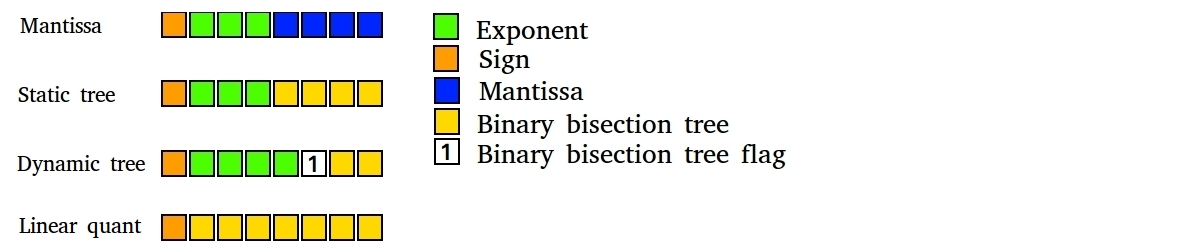
\includegraphics[width=1\linewidth]{types2.jpg}}
	\end{center}
	\caption{Anatomy of the four different 8-bit data types. Note that the dynamic data type shown here is a specific example and the number of bits for exponent and for the tree varies between individual floating point numbers.}
\end{figure}

\subsection{Implementation and computational performance}

The fastest implementation for 8-bit compression and decompression we could think of is to use a binary search on a sorted table of all positive 128 values in shared GPU memory and keep track of the sign of the respective number. Shared memory is about 100 times faster than global GPU memory and thus a binary search in shared memory is very fast. 

In our implementation we used one thread per number in a binary search. Additional parallelization is easily possible by dividing the table into $n$ intervals, where $n$ is the number of threads per number. However, the necessary thread synchronization is expensive and performance gains are probably negligible compared to the additional resource costs (threads). 

For decompression the table is read into shared memory and a lookup is performed for the 32-bit value for the respective 8-bit value. Here we use one thread per number/lookup.

On average, these algorithms perform compression and decompression in 1 and 0.5 nanoseconds per number, respectively, as measured on a NVIDIA GTX Titan.

Implementations of our 8-bit approximation algorithms are available online \footnote{https://github.com/TimDettmers/clusterNet/; contact me if you need help with integrating the functions into your library}.

\subsection{Speedup}

We measured the average total transfer time (compression, transfer, and decompression) for our techniques and compared them to 32-bit transfers between GPUs (see Figure 2). We measured this time on a board equipped with 4 GPUs which yields 8 PCIe 3.0 lanes for each GPUs and thus a theoretical bandwidth of about 8GB/s; however, bandwidth for small messages is usually considerably lower. The algorithms were run on two NVIDIA GTX Titans. Each matrix was transfered 100 times and the average total transfer time was measured.

We used the message passing interface (MPI) implementation provided by OpenMPI 1.8.5 which uses low level NVIDIA routines to enable GPU-to-GPU communication without the help of the CPU. MPI is commonly used to parallelize algorithms on GPU clusters.

Using 8-bit approximation is slow for small matrices with less than 50k parameters per layer (see Figure 2) because compression and latency dominate the transfer time.\\
For messages which are larger than 250k parameters per layer, a 2x speedup in transfer speed can be achieved with 8-bit approximation compared to 32-bit data transfers. For smaller matrices, the speedup is exponentially decreasing but 8-bit transfers are always faster than 32-bit transfers.


\subsection{Approximation error}

We tested the approximation error of our data types on multiple distributions and on the gradients (data parallelism) and activations (model parallelism) on MNIST. We calculated the mean absolute and relative error from a sample of size 25 million numbers drawn from normal distributions $N(\mbox{mean},\mbox{variance})$, and the uniform distribution $U(0,1)$. The approximation of $N(0,10^2)$ was done by using an exponent offset of $10^2$ while other numbers used an exponent offset of $10^1$. For the dynamic tree and linear quantization the sample was normalized by division by the maximum absolute value and then denormalized after compression. \\\\
As one can see from Table 1, the 8-bit dynamic tree provides the overall best performance for approximation numbers for random distributions and for parallelism on MNIST. \\\\
For our tests on MNIST we used rectified linear units, a 784x1024x1024x10 architecture with dropout (0.2,0.3,0.3), a learning rate of 0.003 and RMSProp  \citep{tieleman2012lecture}. Usually we have 8-bit approximation for all incoming GPUs and 32-bit gradients for the local GPU.
\begin{figure}[t]
	\begin{center}
		%\framebox[4.0in]{$\;$}
		\fbox{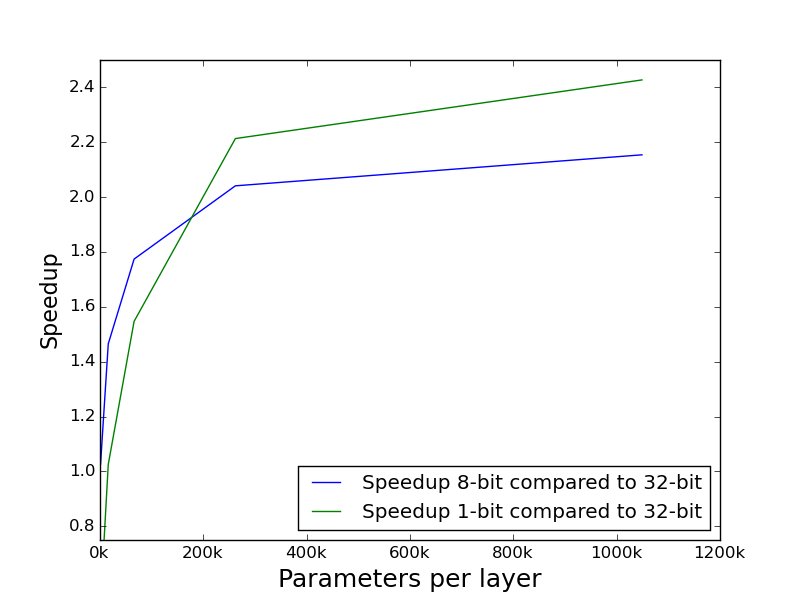
\includegraphics[width=0.8\linewidth]{bandwidth_raw_32vs8vs1_speedups.png}}
	\end{center}
	\caption{Average transfer time for 1-bit quantization and 8-bit approximation compared to 32-bit transfers.}
\end{figure}
In the following experiments we simulated training on a large GPU cluster by only using the pure 8-bit approximation gradient component by training on a single GPU -- so no 32-bit gradients or activations where used. \\
We found that the best test error of all four approximation techniques, static tree, dynamic tree, linear quantization, and mantissa  did not differ from the test error of 32-bit training for both data parallelism $F(4,4) = 0.71, p = 0.59$, and model parallelism $F(4,4) = 0.54, p = 0.71$ (test assumptions were satisfied); also the 99\% confidence intervals did overlap for all techniques. Experiments with logistic units revealed the same results. This indicates that on MNIST 8-bit approximation does not degrade classification performance compared to 32-bit and all 8-bit approximation techniques are similar in performance on MNIST for both model and data parallelism.


\begin{table}[h]
	\caption{Approximation errors on different data sets, and for different layers.}
	\label{sample-table}
\begin{minipage}
	{\linewidth}
	\centering
	\begin{tabular}{ cccc}
		\toprule[1.5pt]
		Distribution & Data type & Mean absolute error & Mean relative error in \%\\\midrule
		$U(0,1)$ & 8-bit dynamic tree & {\bf0.00004} & {\bf 1.39}  \\
		- & 8-bit linear quant & 0.0024 & 2.16\\
		- & 8-bit mantissa & 0.0017 & 7.22\\
		- & 8-bit static tree & 0.0007 & 4.82\\\midrule	
		$N(0,1)$ & 8-bit dynamic tree & 0.0005 & {\bf2.46}\\
	- & 8-bit linear quant &  {\bf0.0004} & 6.47 \\
	- & 8-bit mantissa & 0.0104 & 6.89 \\
	- & 8-bit static tree & 0.0093 & 6.3 \\\midrule
	$N(0,10^2)$ & 8-bit dynamic tree & 0.049 & {\bf2.49} \\
- & 8-bit linear quant & {\bf0.041 }& 6.44 \\
- & 8-bit mantissa & 1.066 & 7.19\\
- & 8-bit static tree & 0.926 & 6.28 \\\midrule
$N(0,0.2^2)$ & 8-bit dynamic tree & 0.000018 & {\bf2.45} \\
- & 8-bit linear quant &{\bf 0.000015} & 6.15 \\
- & 8-bit mantissa & 0.00055 & 8.26\\
- & 8-bit static tree & 0.00022 & 6.58 \\\midrule
MNIST model parallel & 8-bit dynamic tree & {\bf 0.025$\>$/$\>$2$\>$/$\>$3321 }& {\bf0.5/2/2} \\
- & 8-bit linear quant & 0.02$\>$/$\>$2.6$\>$/$\>$3387 & 1/2/3 \\
- & 8-bit mantissa & 1$\>$/$\>$70$\>$/$\>$265000  & 1.5/2/8\\
- & 8-bit static tree & 0.45$\>$/$\>$50$\>$/$\>$187000 &  1/2/6 \\\midrule
MNIST data parallel & 8-bit dynamic tree & {\bf 0.0005$\>$/$\>$0.004$\>$/$\>$0.95} &  {\bf3/4/5} \\
- & 8-bit linear quant & 0.001$\>$/$\>$0.01$\>$/$\>$1.25 & 5/6/6 \\
- & 8-bit mantissa & 0.02$\>$/$\>$0.1$\>$/$\>$55 & 4.5/4.5/6\\
- & 8-bit static tree & 0.01$\>$/$\>$0.04$\>$/$\>$24&  4/4/5\\
\bottomrule[1.25pt]
\end{tabular}
\par
\bigskip
\end{minipage}
\end{table}

We also tested our data types on CIFAR10 where we used a convolutional network\footnote{http://code.google.com/p/cuda-convnet/wiki/Methodology} with two convolutional layers (64x5x5, 64x3x3), which were followed by max-pooling (3x3) and contrast normalization after each layer. These layers were followed by two locally connected layers (no weight sharing) and a final fully connected softmax layer.

We used both data parallelism (convolutional layers) and model parallelism (local layers) for this convolutional net and we found that test errors for all 8-bit data types and 32-bit training only differed by at most 2\% relative to each other, indicating that 8-bit approximation did not decrease performance.

We also applied to 8-bit dynamic tree data type to AlexNet on the ImageNet dataset. We used our approximation scheme for both model (dense layers) and data parallelism (convolution). 

\begin{figure}[h]
	\begin{center}
		%\framebox[4.0in]{$\;$}
		\fbox{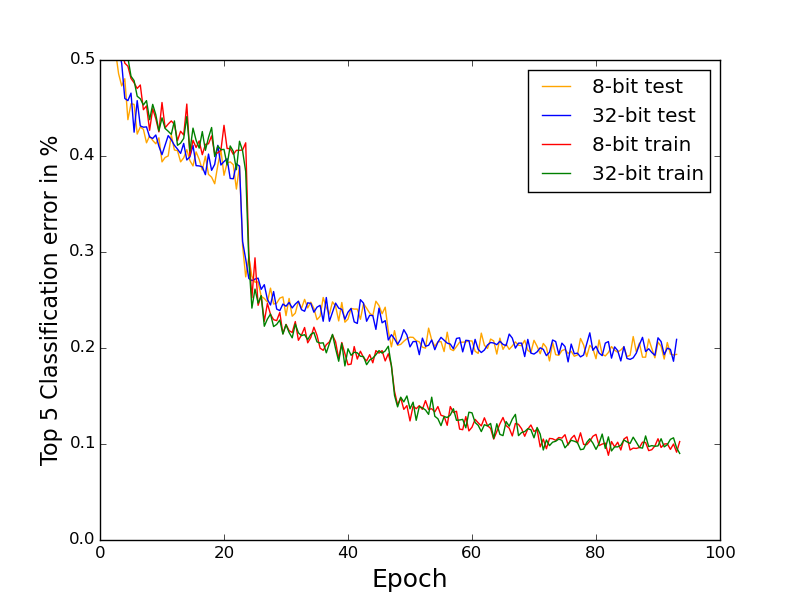
\includegraphics[width=0.7\linewidth]{imagenet_32vs8.png}}
	\end{center}
	\caption{Classification train and test error for the 8-bit dynamic data type used in AlexNet on the ImageNet dataset.}
\end{figure}

Figure 3 shows that the 8-bit dynamic tree data type does not increase the misclassification error on the train or test set for convolutional nets. The final performance on the test set was comparable to the 32-bit model: 18.65\% and 18.55\% Top5-test-error for the 8-bit and 32-bit model, respectively.

\subsection{Improved performance}
\begin{figure}[h]
	\begin{center}
		%\framebox[4.0in]{$\;$}
		\fbox{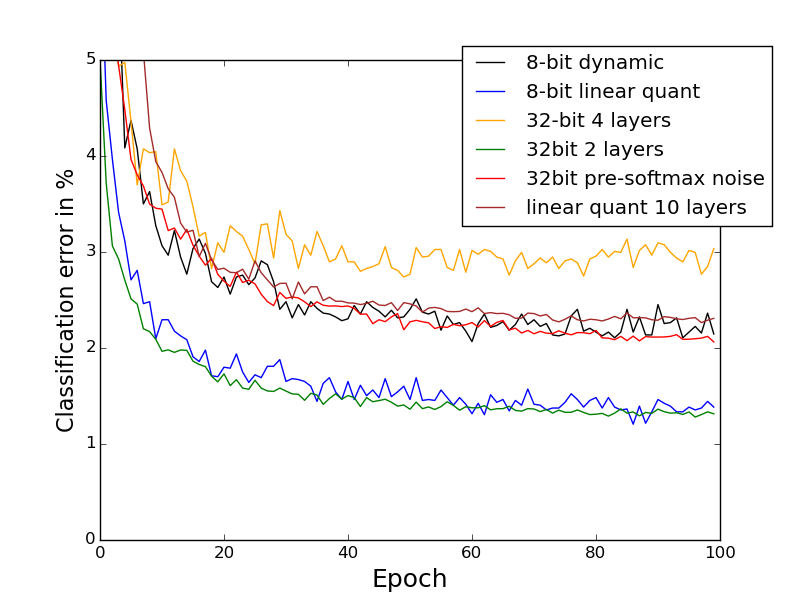
\includegraphics[width=0.7\linewidth]{deep_faster.png}}
	\end{center}
	\caption{Average misclassification error on MNIST over 8 runs (2 runs for 10 layers) for model parallelism for 32-bit vs 8-bit neural networks with 4 hidden layers and RMSProp.}
\end{figure}

Figure 4 shows the average error of deep networks  which were trained with either 32-bit or 8-bit model parallelism. We found that the mantissa and static tree data types are unstable due to high errors rates which accumulate during model parallelism. We were unable to train a 10 layer networks (gradient clipping would be needed) and 4 layers diverge often despite low learning rates. The dynamic and linear quantization data types on the other hand, were stable due to lower errors and their inherent dynamics.\\\\
We observed an interesting phenomenon which was also observed by \citet{seide20141} where the approximation can make learning faster and {\it improve} classification performance. We found similar results in model parallelism (see Figure 4), where we could train 4 layer and 10 layer networks significantly faster than with 32-bit activations. This is a reliable effect ($t(7) = 19.3, p < 0.001$) which in this case allows 4 hidden layers of size 1024 to be trained as fast as a network with two hidden layers which used 32-bit activations; and a network with 10 hidden layers faster than a network with 4 hidden layers using 32-bit activation. In comparison, a network of 10 hidden layers trained with 32-bit did not surpass 30\% cross validation error and was highly unstable. We did not observe this effect for data parallelism and networks with only 2 hidden layers.\\\\
We tested the same procedure without using RMSProp and this behavior disappeared and we can thus conclude that this behavior is partially due to RMSProp (\citet{seide20141} used Adagrad). Further experiments showed that, (1) the effect is not due to the learning rate and (2) not due to the truncation of small activation during normalization by the maximum absolute value. Using noise which is proportional to the relative approximation error of linear quantization, we could replicate the effect partially (see 32bit pre-softmax noise in Figure 4) by applying the noise after dropout while leaving the activation, used during backpropagation, untouched. We found that this effect was largest when applied to the last layer before the softmax. Further analysis showed, the combination of RMSProp and linear quantization increases sparsity of activations in hidden layers by about 40\%, and decreases sparsity by a factor of two in the final hidden layer. This effect was not observed when we applied proportional random noise. We reasoned that correlated noise per class would come closer to the effect of linear quantization, but the results were similar to using the random, proportional noise. As such we conclude that the effect of improved performance in deep networks is due to the internal dynamics of RMSProp and linear quantization themselves.
\section{Comparison to other methods}

\subsection{Dynamic fixed point}

Dynamic fixed point data types are data types which use all their bits for the mantissa and have an dynamic exponent which is kept for collection of numbers (matrix, vector) and which is adjusted during run-time. \citet{courbariaux2014low} used dynamic fixed point data types with 10-bit width for computation and 12-bit width for parameter updates to train a maxout convolutional networks end-to-end. Their results on PI MNIST, MNIST, and CIFAR10 are about 20\% worse relative to the state of the art obtained by \citet{goodfellow2013maxout}.\\ 
In our work we shows that we can use 8-bit gradients for our parameter updates without degrading performance. However, dynamic fixed point data types can also be used for end-to-end training and as such a combination of both methods might yield optimal performance. 

\subsection{1-bit quantization}
A technique comparable to 8-bit approximation is 1-bit quantization which was developed by \citet{seide20141}: In 1-bit quantization each 32-bit number of the gradient is quantized to a single bit by a quantization function. This quantization function maintains a cumulative quantization error which is used by the quantization function to smoothen out error over time. The immediate error in quantization is too high to produce stable and accurate forward passes for model parallelism, but in data parallelism 1-bit quantization will converge to a local minimum seamlessly. To attain global quantization information, the procedure quantizes gradients twice by accumulating parts from different GPUs and thus overhead and latency of quantization and transfers are larger for this technique compared to the single pass for 8-bit approximation, which might create problems for larger computer networks.

In our comparison we used the 1-bit quantization implementation of Torch7\footnote{https://github.com/facebook/fbcunn} \citep{collobert2011torch7}. The measurement then followed the same procedure as in the 8-bit case in section 3.3 where mean total transfer time was measured.

For large matrices with more than 300k parameters, 1-but quantization is about 10-20\% faster than 8-bit approximation (see Figure 2), while 8-bit approximation is notably faster for layers with less than 200k parameters like those found in the first layers of convolutional networks or during model parallelism. However, while 1-bit quantization only works for data parallelism, 8-bit approximation also works for model parallelism which is fundamental for achieving high performance implementations of convolutional nets (Krizhevsky 2014). 

So 1-bit quantization will be more efficient for large scale GPU clusters that train large dense neural networks, while 8-bit approximation will perform favorably for convolutional nets and is also usable for model parallelism. A combination of these techniques would also be useful, with 1-bit quantization in data parallel convolutional layers and 8-bit approximation in model parallel dense layers of a convolutional net. 

\section*{Conclusion}

Here we have shown that approximation of 32-bit floating point numbers with 8-bits can speed up communication in parallel training of deep learning architectures by a factor of two relative to 32-bit communication while retaining or even improving predictive performance. We have shown that the dynamic tree data type is able to approximate random numbers better than other data types, but that during training all approximation techniques seem to perform equally well. We also showed that 8-bit approximation compares favorably with 1-bit quantization.

We expect that further important advances in parallel computing for deep learning will come from new hardware (3D GPU memory, EDR InfiniBand adoption) and new algorithms which maintain the performance of backpropagation while providing qualities which make them easier to parallelize. 

\bibliography{iclr2016_conference}
\bibliographystyle{iclr2016_conference}

\end{document}
